% by Mirella M. Moro; version: January/18/2012 @ 04:16pm
% -- 01/18/2012: more discussion on SBBD + JIDM; overall revision
% -- 09/03/2010: bib file with names for proceedings and journals; cls with shrinked {received}
% -- 08/27/2010: appendix, table example, more explanation within comments, editors' data

\documentclass[jidm,a4paper]{jidm} % NOTE: JIDM is published on A4 paper
\usepackage{graphicx,url}  % for using figures and url format
\usepackage[T1]{fontenc}   % avoids warnings such as "LaTeX Font Warning: Font shape 'OMS/cmtt/m/n' undefined"
\usepackage[utf8]{inputenc}

%\usepackage{cite} % NOTE: do **not** include this package because it conflicts with jidm.bst

% Standard definitions
\newtheorem{theorem}{Theorem}[section]
\newtheorem{conjecture}[theorem]{Conjecture}
\newtheorem{corollary}[theorem]{Corollary}
\newtheorem{proposition}[theorem]{Proposition}
\newtheorem{lemma}[theorem]{Lemma}
\newdef{definition}[theorem]{Definition}
\newdef{remark}[theorem]{Remark}

% New environment definition
\newenvironment{latexcode}
{\ttfamily\vspace{0.1in}\setlength{\parindent}{18pt}}
{\vspace{0.1in}}

% ALL FIELDS UNTIL BEGIN{document} ARE MANDATORY

% The following data (volume, number and page) are given by the editors prior to publishing your article
\jidmVolume{5}
\jidmNumber{1}
\jidmYear{14}
\jidmMonth{June}
\setcounter{page}{1}


% Includes headers with simplified name of the authors and article title
\markboth{R.M.C. Segundo, M.N. Amorim, C.A.S. Santos}
{JIDM - Journal of Information and Data Management}
%  -> \markboth{}{}
%         takes 2 arguments
%         ex: \markboth{M. M. Moro}{Any article title}


% Title of the article
\title{LiveSync: a method for Real Time Video Streaming Synchronization from Independent Sources}


% List of authors
%IF THERE ARE TWO or more institutions, please use:
%\author{Name of Author1\inst{1}, Name of Author2\inst{2}, Name of Author3\inst{2}}
\author{Ricardo M. C. Segundo\inst{1}, Marcello N. de Amorim\inst{2}, Celso A. S. Santos\inst{3}}


%Affiliation and email
\institute{Federal University of  Espirito Santo, Brazil  \\ \email{rmcs87@gmail.com , novaes@inf.ufes.br , saibel@inf.ufes.br}
% IF THERE IS ANOTHER INSTITUTION:
%\and Name_of_the_second_institution \\
%\email{address@whatever.com}
}


% Article abstract - it should be from 100 to 300 words
\begin{abstract}
This work presents a tool that allows users to synchronize live videos from multiple sources such as YouTube or any other video streaming sources. The proposed approach to proceed the multiple camera video synchronization is based in crowdsourcing techniques, using the power of a crowd of collaborators to synchronize videos, requiring from each user the sync of only a pairs of videos. Additional sync relations are inferred from the known contributions, using transitivity properties and an appropriate structure for this inference, the Dynamic Alignment List.
\end{abstract}


% ACM Computing Classification System categories
\category{H.4.4.3}{Information Systems Applications}{Crowdsourcing} 
\category{H.3.2.7}{Human-Centered Computing}{Synchronous editors}

% Categories and Descriptors are available at the 1998 ACM Computing Classification System
% http://www.acm.org/about/class/1998/
%  -> \category{}{}{}
%         takes 3 arguments for the Computing Reviews Classification Scheme.
%         ex: \category{D.3.3}{Programming Languages}{Language Constructs and Features}
%                   [data types and structures]
%                   the last argument, in square brackets, is optional.

% Article keywords
\keywords{live video, synchronization, crowdsourcing}
%  -> \keywords{} (in alphabetical order \keywords{document processing, sequences,
%                      string searching, subsequences, substrings})


% THE ARTICLE BEGINS
\begin{document}

% This is optional:
\begin{bottomstuff}
The authors would like to thank the "Fundação de Amparo à Pesquisa e Inovação do Espírito Santo" (FAPES) and "Coordenação de Aperfeiçoamento de Pessoal de Nível Superior" (CAPES) for financial support.
\end{bottomstuff}

\maketitle

\section{Introduction}
This paper extends the previous work \cite{delivesync} that won the prize of best tool in the XVI Workshop on Tools and Applications (WFA) of the XXII Brazilian Symposium on Multimedia and Web Systems (WebMedia 2016).

Multiple camera video synchronization is a research area within multimedia. Automatic video synchronization (AVS) is a form to synchronize multiple video streams. AVS can be done analysing video segments \cite{wang2014videosnapping} or audio ones \cite{su2012making}. In Schweiger et.al.\cite{schweiger2013fully} we find these and other approaches in the area. One main contribution of this paper is the description of the challenges for automatic synchronization algorithms: wide baselines, camera motion, dynamic backgrounds and Occlusions.

We propose in this work the use of crowdosurcing techniques to synchronize these videos, instead of an automatic one. Crowdsourcing\cite{howe2006rise} in our scope refers to the use of the crowd as part of a computational problem that can be solved easily by a human than by a machine. The "easily" word can mean that the human approach: is cheaper, faster or can be done more efficiently by humans.

In video synchronization, we know that humans can ful- fil all challenges presented by \cite{schweiger2013fully}. A person can identify if two videos are synchronized or not independently of occlusions, change of the background, camera motion or view point changes. The main challenge is how to use the human abilities to synchronize the videos, and permit that other persons can benefit from these contributions. So our tool uses the power of the crowd to synchronize live streaming videos and provide a form that other persons that want to watch those videos can receive both videos and synchronization info.

The remaining of this paper is presented as follows: section 2 explains our approach to synchronize videos; section 3 details our tool; section 4 presents a larger experiment to validate our tool in a more comprehensive application scenario ;and section 5 presents our final remarks.






\section{LiveSync}
Live synchronization includes the scenario where a viewer has access to an event that is live streamed by more than one Content Provider. These content providers are independent, so their videos do not have initial resources that allow their automatic synchronization to viewers, requiring a video analysis to generate synchronization points (Couplers). This synchronization fits as a problem that can be solved by using the power of the crowd. This occurs because videos are generated independently, without synchronization points and without previous description of what is about to be shown in screen, neither how can it be correlated to other videos. This way, human perception is used in real time to generate unknown synchronization points. 

As example for this scenario, we can take a public manifestation. In the event, multiple people can take their cell phones and start streaming the event. In their house, other people can watch the videos. However, the multiple videos from different sources will be asynchronous. We need a way to synchronize these UGV. We use the crowd to achieve it. To this objective we group all videos in a MashUp application that connects to a Coupler Server that contains all synchronization data. Both synchronizing and playing the videos are made using this mashup, that can receive videos from multiple sources.






%%%%%%%%%%%%%%%%%%% ACM %%%%%%%%%%%%%%

Live synchronization includes the scenario where a viewer has access to an event that is live streamed by more than one Content Provider. These content providers are independent, so their videos do not have initial resources that allow their automatic synchronization to viewers, requiring a video analysis to generate synchronization points (Couplers).

As example for this scenario, we can take a public manifestation. In the event, multiple people can take their cell phones and start streaming the event. In their house, other people can watch the videos. However, the multiple videos from different sources will be asynchronous. We need a way to synchronize these UGVs. We use the crowd to achieve it. To this objective we group all videos in a mashup application that connects to a Coupler Server that contains all synchronization data. Both synchronizing and playing the videos are made using this mashup, that can receive videos from multiple sources.

In a live presentation, it is assumed that content must be consumed right after its generation. It is of extreme importance that the synchronization method can be performed in playback time, to allow the integration of live content. However, not all viewers are required to be part of the crowd to achieve synchronization. If a synchronization made by a single member of the crowd is accepted as accurate, it can be transferred to the remaining viewers, this way each one will have his content locally synchronized.

One way of live synchronization can work is as follows: a person selects and synchronizes two videos with the help of a manipulation tool. This becomes a candidate synchronization point. Several people can do the same, and the results can be based on multiple synchronizations. Having these synchronization points defined, synchronization information can be sent to other viewers interested in watching those videos. As simple example, take two independent sources that are transmitting an event. A mashup system allows the user to watch both videos at the same time is his device. However the videos are asynchronous and the user notices that. He then access the option to synchronize the videos. After he achieve a synchronous result, implicitly his contribution is sent to a server that will feed other users that choose to watch the same videos with the synchronization specification. If the user thinks the content is not synchronised yet, he can synchronize it himself and send another contribution. This tool was implemented and is presented on section~\ref{livesync}.







\section{LiveSync Tool}
The LiveSync Tool is a Web implementation for the LiveSync, it provides all components required to proceed UGV live stream synchronization following the LiveSync method. Moreover, the LiveSync Tool also provides an implementation for Dynamic Aligned List (DAL), the abstract datatype used to register and manage the user contributions.


\subsection{Remote Temporal Couplers (RTC)}
LiveSync is based on the previous technique Remote Temporal Couplers (RTC) \cite{segundo2015remote} that intents to synchronize multiple contents related to the same main-content (MC). These contents may come from different Content Suppliers (CS), and range from video objects to extra content (EC), such as subtitles, additional information boards, labels, audio objects, or any other media artifacts that can me aligned over the same timeline.

RTC is based on three components: Main Content Provider, Content Suppliers, and User Devices (UD). Figure~\ref{rtc} \cite{segundo2015remote} shows the communication between these three components.

\begin{itemize}

\item \textit{MC Provider} is responsible for streaming the MC, that usually is a video stream transmitted over accessible channels to UD and CS.

\item \textit{Content Suppliers} provide EC related to a MC requested by UD. 

\item \textit{User Devices} are responsible to control one or more services provided by CS and playing the MC.
 
\end{itemize}


\begin{figure}[h!]
	\centering
	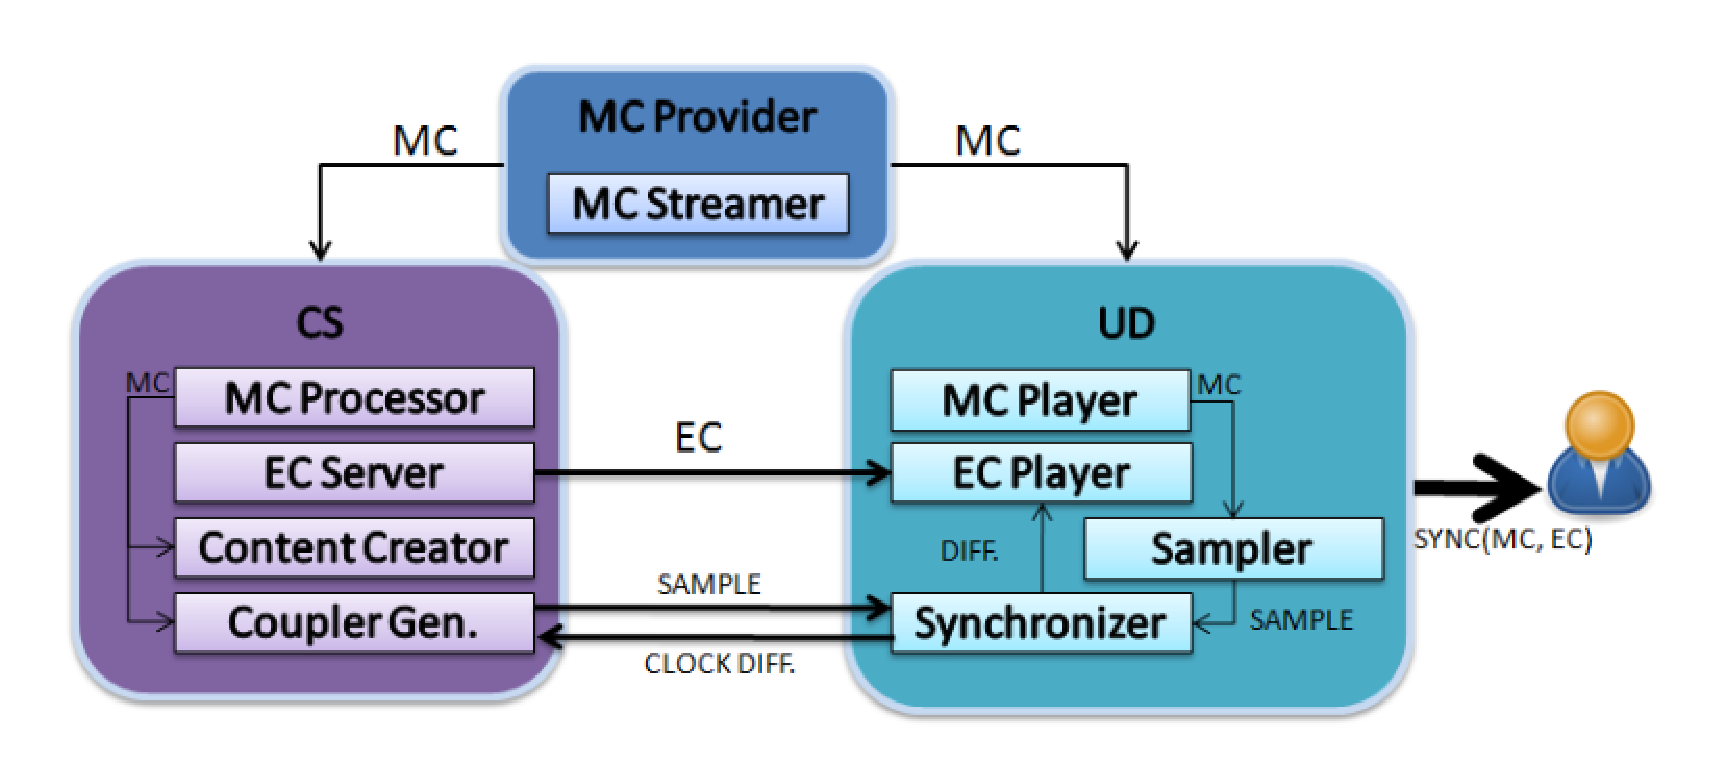
\includegraphics[scale=0.4]{figures/rtc}
	\caption{RTF - Entities Composition for Content Synchronization}
	\label{rtc}
\end{figure}

RTC consider that MC Providers usually offers no explicit timing information in its content to support the synchronization. Although, CS can provide synchronized content without depending on a explicit time specification sent by the MC Provider. The way found for reach synchronization into this scenario is delegate to CS the responsibility  for generate temporal couplers. A temporal coupler is an structure that relates a scene to the local timestamp, associated with it on a CS. In other words, for each scene $Sx$ presented by a CS, it provides a temporal coupler \textit{[Sx, Timestamp]} that identifies the local time when the scene occurred in its local timeline.

Finally, the RTC technique uses the timestamp into each temporal coupler to synchronize the contents from multiple Content Suppliers, as well to compose a coherent presentation in a mash-up application, in which users can choose what contents should be included.

Although LiveSync approach to synchronize video streams is based on RTC, it uses relational couplers, instead the temporal couplers used by RTC. A relational coupler relates pairs of videos and the $\Delta{time}$ between them. In this approach, alignment is constructed by relating a set of video streams, pair to pair, to generate coverage on the event timeline, rather than taking on a main-stream and to align each other stream with it. Moreover temporal couplers still are used in LiveSync to correctly play the synchronized streams.











\subsection{Dynamic Aligned List (DAL)}

To achieve video streaming synchronization was used the Remote Temporal Couplers (RTC) technique \cite{segundo2015remote} that allows to align videos from different sources. This technique collects synchronization points for pair of videos, and uses an inference algorithm to find out more relations between videos by transitivity over known relations.






The RTC technique was operationally represented as the Dynamic Alignment List (DAL), an abstract type designed to organize the relations between videos as well provide the functionalists required to store and process the relations.

The start model for the storage structure inside the DAL was a relational matrix MxM which can represent all possible relations between M videos, each position representing the $\Delta{time}$ between the initial point of a pair of videos. This matrix was reduced to a upper triangular matrix because $\forall{i,j} < M , \Delta_{i,j}$ = $- \Delta_{j,i}$ and the main diagonal was eliminated because $\Delta_{i,j}$ is always equal to zero. The $\Delta{time}$ for each couple of videos is calculated for $\Delta{i,j} = start(j) - start(i)$ where $start(X)$ returns the offset of video X from the start of the event's timeline.

These values are used to synchronize the M videos. If $\Delta{i,j} > 0$ the video $i$ starts before the video $j$, if $\Delta{i,j} < 0$ the video $i$ starts after the video $j$, and when $\Delta{i,j} = 0$ both videos start at the same time. The values are represented in milliseconds, so $\Delta{i,j} = 30$ means the video $j$ should starts 30 ms after the video $i$ starts in order to achieve their synchronization. Additionally, in cases which is impossible to determine a relation between a pair of videos, the value registered is $I$ that means impossible.

Into a collaborative scenario where users can contribute providing a $\Delta{i,j}$ for a pair of videos $(i,j)$, it is important to store all contributions, because the $\Delta{time}$ value should be calculated considering the contributions collected for that pair. In that approach the formula $\Delta{i,j} = start(j) - start(i)$  is used to calculate the $\Delta{time}$ for each contribution, and the value stored in DAL is determined processing all contributions for each pair. Moreover, the number of contributions for each pair can grow while the contribution process is active, and current $\Delta{time}$ of a pair can change while contributions are incoming.

In order to represent this model it was needed to define a structure more sophisticated then a matrix. This structure preserves the relational characteristics of a upper triangular matrix without the main diagonal, with an additional dimension related to the contributions for each relation between video pairs. However, it is implemented as a hash table, using linked lists hierarchically organized in three levels. 

\begin{itemize}

\item Level 1 - The first level is a list of video structures. Each structure has a unique identification label for a correspondent video. 

\item Level 2 - Each video structure points to a second level linked list composed by all possible relations that include its video, considering the relations in a upper triangular matrix without the main diagonal.  Thus, each node in a second level linked list corresponds to a relation between it's video represented in its root and another video.

\item Level 3 - Each relation in a level 2 list points to a third level list, in which each node represent a contribution for that relation.

\end{itemize}

Figure~\ref{dal} exemplify a data structure into a DAL with 5 videos. The videos, labeled as $A, B, C, D$  and $E$, are in the fist level linked list. Each video points to a second level list, it is possible to observe in Figure~\ref{dal}  that each second level linked list have only the relations that would exist in a single line of a upper triangular matrix without the main diagonal. Moreover, in Figure~\ref{dal} each relation, that is an element of second level list, points to a cloud that represents a third level list with all contributions for that relation.

\begin{figure}
	\centering
	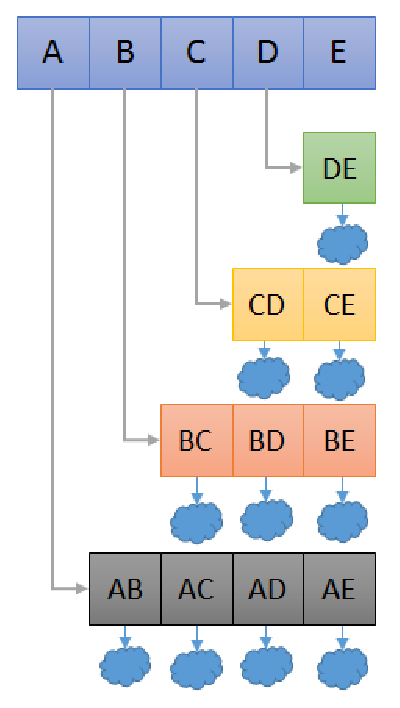
\includegraphics[scale=0.8]{figures/dal}
	\caption{DAL with 5 Videos (A,B,C,D,E)}
	\label{dal}
\end{figure}

A completed DAL can provide all information needed to achieve synchronization for videos registered on it, although it is more than a data structure. DAL is an abstract datatype that provides the data structure plus a set of features that allows access, manage and process the information inside it, such as the function \textit{Infer Synchronization}. 

\textit{Infer Synchronization} can obtain additional relations by executing an inference algorithm over the current relations. This algorithm checks if is possible to find an indirect path between two videos by transitivity. For example, considering the videos $A, B$ and $C$, if the relations $AB$ and $BC$ are known, by transitivity is possible to infer the relation $AC$. This feature can reduce the number of contributions required to complete a DAL. 





\subsection{Main Funcionalities}
The main functionalities provided by or tool are:
\begin{description}
	\item[Synchronized Live Video Player -]	the tool permits users to watch multiple videos synchronized. He selects from a list of sources the videos he wish to watch and them they are synchronized using information provided by other users.
	
	\item[Video Synchronization -] If a pair of videos does not have any information about their synchronization, users are invited to contribute and synchronize the videos.
	
	\item[Infer Synchronization -] In some cases that there is no direct information about the synchronization of two videos, the tool is able to infer the synchronization about them, based on the contributions of other videos. We use the transitive attribute of video synchronizations, where if we know AB and BC synchronization info, we can infer AC. To infer this value we travel trough the DAL, finding the unknown relations (for example, CE), and try to find a path of known relations where we can infer CE. Taking the DAL in Figure~\ref{dal}, we can infer CE if we know: AC and AE. This a two steps rout, but try all possible routes when inferring, in a way that we fill as much relations as possible.
	
	\item[Video Aggregation -]	Although the focus of the LiveSync tool being on synchronization, we allow users to add new stream sources to the application. He only needs to set the video source, and the video will be added to the DAL and list of videos. However, we don't do any filtering about the added video, this means that the user can add any video to the application, even ones that contains none relation with the other videos. In future versions we plan to add options where other users can mark the video as not related, and then remove them.
	
	\item[Multiple Platforms Support -] One keypoint of our tool is the use of other platforms as video sources. The videos that we play to users and that we synchronize, are not provided by us, but by other live video stream platforms. To be compatible with our tool, two requisites are required:
	\begin{enumerate}
		\item Remote Player: we need that the platform allows embeddable player on third pages, allowing us to control the player with its basic functionalities such as: play, pause and stop;
		\item Uptime Support: a second and fundamental requisite is an API that allows us to retrieve the video Uptime. Video uptime is the time since the beginning of the video that is presented on the video player. This is fundamental to create and replicate the couplers generated in synchronization process.
	\end{enumerate}
	
	\item[Serverless Architecture -] Serverless architectures refer to applications that significantly depend on third-party services and putting much of the application behavior and logic on the front end. Such architectures remove the need for the traditional server system sitting behind an application \cite{RobertServerless}. More of this characteristic will be addressed in the next topic: Architecture.
	
	\item[Multiplatform -] LiveSync is a Web Based application designed and developed in compatibility with HTML5 standard to its front-end (MashUp Player) component. It allows our application to run on multiple browsers, operational systems and devices.
	
	\item[Active X Passive Contributions -] Two branches of the LiveSync are currently on our repositories. They differ only in one aspect: who what videos are to be synchronized, the crowd or the application? The active version allows user to navigate freely through the videos, synchronizing them when they wish to. The focus of this branch is to allow users to contribute if they want to. On the other hand, the Passive branch gives the crowd exactly what video they will synchronize. The focus here is to rapidly synchronize all videos, so the focus isn't to make users watch the videos, but force them to synchronize all the base for other porpoises. The active branch is the focus here, but can easily converted to the passive.
	
\end{description}

\subsection{Architecture}
The LiveSync Tool has three main components (Figure~\ref{livesync}): the Content Providers (Video Sources), the Coupler and the Mash-up Player.

\begin{figure}[h]
	\centerline{\includegraphics[scale=0.6] {figures/architecture}}
	\caption{LiveSync Tool's components}
	\label{livesync}
\end{figure}

\subsubsection{Content Providers}
Content Providers are third-parties videos streamers platforms, such as YouTube Live, LiveStream, TwitCast, Twitch and Ustream. LiveSync Tool supports different platforms as video sources, maximizing the number of videos streams that can be related to an event.

There are two requirements that a Content Provider must attend to be compatible with LiveSync: Remote Player and Uptime Support.

As each flow platform uses its own protocols, the embedded players are required for aggregation in the mash-up application. These players must provide buttons to play, pause and stop actions.

Uptime Support, is necessary to find the temporal couplers to video streams. Uptime is the time passed since the beginning of the live stream until the video part being presented in the player at the moment of the call.


\subsubsection{Coupler Service}
The Coupler Service (CS) is responsible for storage, distribution and calculation of synchronization points between video streams from the Content Providers. Coupler Service provides a DAL instance and Log files. 


%This goes in direction of the Serverless Architecture. 



%We wanted an architecture that needed low resources (another justification for using third party stream services) and easy deployment. All that is necessary do execute the CS is a NODE.JS (https://nodejs.org/en/) server instance. This is possible because the CS is fully developed in JavaScript and compatible with the HTML5 standards. To deploy the CS, we use a Backend as a Service or ”BaaS” platform, more specifically we use the Heroku (www.heroku.com) one, that permits free use of NODE.JS instances.


It stores synchronization information only during the duration of the event, so its stance is finished with the end of the videos and all data is lost. In the current scope, the sync info is only necessary during the event, after it, there is no need to store the information. For reasons of testing and using the filmed videos from YouTube was generated log files that contains all contributions made by the crowd. If it is important to maintain all contributions and data for post analyses and further use, unstable version of the LiveSync is being configured to use a fully transactional database.  A fully transactional database is used to track all contributions made by the crowd, an important aspect for crowdsourcing support and that is also supported by the DAL.

Other aspect of the CS is that it is responsible for the distribution of relational couplers, containing synchronization information between pairs of video streams. When an user selects a pair of streams, a message is sent from the mash-up to CS, containing the required relation. CS then answers it with required information. If the relation is unknown, it responds with a prompt for the user to synchronize them.

The last functionality on Coupler Service, is to calculate the synchronization points between videos streams. Each relation ($\Delta_{A,B}$) may contain several contributions, then it is necessary to calculate a value to that relation based on the contributions. In the current version, this delta is calculated by the geometric mean of the contributions to find an satisfying value. CS also uses the Inference functionality by DAL to find additional relations over these calculated values.

The communication  between CS and the mash-up application is made through Websocket communication. The mash-up application creates a WebSocket channel to CS, and requests the sync information or sends contributions from the crowd. A simple protocol is used for JSON messages: {act:value, data:object}. The \textit{act} field contains the action to be made and the \textit{data} field contains an object to complement the action. As example, the action used to send a new contribution, transmit as value for its \textit{data} field a relational coupler representation that contains the videos involved, as so the contribution value for the $\Delta$ between them.



\subsubsection{Mash-up Player}
Mashups are applications generated by combining content, presentation or other applications functionalities from disparate sources. They aim to combine these sources to create useful new applications or services (the offer and consumption of data between two devices) to users \cite{yu2008understanding}. In LiveSync we combine videos coming from different sources and platforms with the synchronization information from the coupler to reproduce a synchronous presentation of these videos.

The MashUp Player is responsible for both presenting video synchronously and collecting the synchronization. Figure~\ref{screen1} represents the interface of the MashUp.

\begin{figure}[h]
	\centerline{\includegraphics[scale=0.3] {figures/screen}}
	\caption{Modelo simplificado do live-sync}
	\label{screen1}
\end{figure}

On the top we have all information necessary to the user. He can aggregate new videos using the ADD NEW VIDEO options, SYNCHRONIZE the videos if he thinks the videos are not synchronized or he can just select the videos he want to watch. When just playing two selected videos from the videos list, each video player creates an instance for the player that is compatible with that source (YouTube or WebSocket). It is invisible to the user where the video is coming from.

When the user adds a video, an input text is shown to him, and he can add the video URI (WebSocket) or video ID (YouTube). The page reloads and the new video is listed in the video list for every one that connects to the application. When the video is added by the user, an message is sent to the Coupler, containing the action to add a new asset to the DAL, and the specification of it, such as label and URI.

The last functionality of the MasUp is to synchronize the videos. When the user clicks on SYNCHRONIZE, a new mode of the application is revelled showing the synchronization tools. We use a Play 'n Pause approach to synchronize the videos. After he thinks the videos are synchronized, clicking the DONE button, his contributions is sent to the Coupler and stored in the DAL for further processing of the relation.

\paragraph{Play 'n Pause}
If two videos with a certain degree of similarity, are presented to an individual from the crowd, he can possibly notice that one video is ahead of the other. This way, he can pause the video that is ahead on time while the other remains playing, until reaching a point of synchronization. Then, the user can resume playback of the first video. This process can be repeated until an individual feels like both videos are being presented synchronously.

\section{Case Study}
The case study chosen to validate LiveSync, as well LiveSyncTool, was an internal event that could be streamed by volunteers through their smartphones. This event consisted in [XXXXXXXXXXXXXXXXXXXXXXX].


\section{Final Remarks}
The LiveSync tool allows users to watch live video streams from multiple sources synchronized. If the videos are not synchronized, user can contribute and synchronize them- selves the videos and help building the synchronization, in a crowdsourced approach, believing that using human perception is better than using automatic approaches in this specific case.

Our tool however presents some limitations that shall in the futures be suppressed, such as the number of events that we can follow. Now, each instance of Coupler and MashUps can handle only one event, in other words, we can not cover two independent live events at the same time with one instance, for that porpoise we need more than on instance of each service. Also, new stream services must be added to increase our compatibilities.

Github \url{https://github.com/rmcs87/liveSync} contains all code for LiveSync.

\bibliographystyle{jidm}
\bibliography{jidm}

\end{document}

